\documentclass{beamer}
\usepackage[utf8]{inputenc}
\usetheme{Madrid}
\usecolortheme{default}
\usepackage{amsmath,amssymb,amsfonts,amsthm}
\usepackage{txfonts}
\usepackage{tkz-euclide}
\usepackage{listings}
\usepackage{adjustbox}
\usepackage{array}
\usepackage{tabularx}
\usepackage{gvv}
\usepackage{lmodern}
\usepackage{circuitikz}
\usepackage{tikz}
\usepackage{graphicx}
\setbeamertemplate{page number in head/foot}[totalframenumber]
\usepackage{tcolorbox}
\tcbuselibrary{minted,breakable,xparse,skins}
\definecolor{bg}{gray}{0.95}
\DeclareTCBListing{mintedbox}{O{}m!O{}}{%
breakable=true,
listing engine=minted,
listing only,
minted language=#2,
minted style=default,
minted options={%
linenos,
gobble=0,
breaklines=true,
breakafter=,,
fontsize=\small,
numbersep=8pt,
#1},
boxsep=0pt,
left skip=0pt,
right skip=0pt,
left=25pt,
right=0pt,
top=3pt,
bottom=3pt,
arc=5pt,
leftrule=0pt,
rightrule=0pt,
bottomrule=2pt,
toprule=2pt,
colback=bg,
colframe=orange!70,
enhanced,
overlay={%
\begin{tcbclipinterior}
\fill[orange!20!white] (frame.south west) rectangle ([xshift=20pt]frame.north west);
\end{tcbclipinterior}},
#3,
}
\lstset{
language=C,
basicstyle=\ttfamily\small,
keywordstyle=\color{blue},
stringstyle=\color{orange},
commentstyle=\color{green!60!black},
numbers=left,
numberstyle=\tiny\color{gray},
breaklines=true,
showstringspaces=false,
}

\title
{4.13.47}
\date{September 30, 2025}
\author
{EE25BTECH11043 - Nishid Khandagre}

\begin{document}

\frame{\titlepage}

\begin{frame}{Question}
The ends $\vec{A}$, $\vec{B}$ of a straight line segment of constant length $c$ slide upon the fixed rectangular axes $OX$, $OY$ respectively. If the rectangle $OAPB$ be completed, then show that the locus of the foot of perpendicular drawn from $\vec{P}$ to $\vec{AB}$ is $x^{\frac{2}{3}} + y^{\frac{2}{3}} = c^{\frac{2}{3}}$.
\end{frame}

\begin{frame}{Theoretical Solution}
Given
\begin{align}
\vec{A} &= \myvec{a\\0} \\
\vec{B} &= \myvec{0\\b}
\end{align}
Since $OAPB$ is a rectangle, the opposite corner $\vec{P}$ is:
\begin{align}
\vec{P} &= \vec{A} + \vec{B} \\
&= \myvec{a \\ b}
\end{align}
\end{frame}

\begin{frame}{Theoretical Solution}
$\vec{B}-\vec{A}$ has fixed length of $c$
\begin{align}
\norm{\vec{B}-\vec{A}}^2 &= \myvec{\vec{B}-\vec{A}}^\top\myvec{\vec{B}-\vec{A}} \\
c^2&= a^2+b^2
\end{align}
Let $\vec{H}$ be the foot of the perpendicular from $\vec{P}$ to the line through $\vec{A}$ in the direction $\vec{B}-\vec{A}$.
\begin{align}
\vec{H} &= \vec{A} + \lambda\myvec{\vec{B}-\vec{A}} \\
\lambda &= \frac{\myvec{\vec{P}-\vec{A}}^\top\myvec{\vec{B}-\vec{A}}}{\myvec{\vec{B}-\vec{A}}^\top\myvec{\vec{B}-\vec{A}}}
\end{align}
\end{frame}

\begin{frame}{Theoretical Solution}
\begin{align}
\vec{P}-\vec{A} &= \myvec{\vec{A}+\vec{B}}-\vec{A} \\
&= \vec{B}
\end{align}
So,
\begin{align}
\lambda &= \frac{\vec{B}^\top\myvec{\vec{B}-\vec{A}}}{\myvec{\vec{B}-\vec{A}}^\top\myvec{\vec{B}-\vec{A}}} \\
&= \frac{\vec{B}^\top\vec{B}-\vec{B}^\top\vec{A}}{a^2+b^2}
\end{align}
\end{frame}

\begin{frame}{Theoretical Solution}
We know
\begin{align}
\vec{B}^\top\vec{A}&=0\\
\vec{B}^\top\vec{B}&=b^2
\end{align}
\begin{align}
\lambda &= \frac{b^2}{a^2+b^2}
\end{align}
\end{frame}

\begin{frame}{Theoretical Solution}
Now compute $\vec{H}$:
\begin{align}
\vec{H} &= \vec{A} + \frac{b^2}{a^2+b^2}\myvec{\vec{B}-\vec{A}}\\
&= \myvec{a\\0} + \frac{b^2}{a^2+b^2}\myvec{-a\\b} \\
&= \myvec{a - \frac{ab^2}{a^2+b^2} \\ \frac{b^3}{a^2+b^2}} \\
&= \myvec{\frac{a(a^2+b^2)-ab^2}{a^2+b^2} \\ \frac{b^3}{a^2+b^2}} \\
&= \myvec{\frac{a^3}{a^2+b^2} \\ \frac{b^3}{a^2+b^2}}
\end{align}
\end{frame}

\begin{frame}{Theoretical Solution}
Let $\vec{H} = \myvec{x\\y}$. Then,
\begin{align}
x &= \frac{a^3}{a^2+b^2} \\
y &= \frac{b^3}{a^2+b^2}
\end{align}
Using the constraint $a^2+b^2=c^2$:
\begin{align}
a^3 &= x(a^2+b^2) = xc^2 \\
b^3 &= y(a^2+b^2) = yc^2
\end{align}
\end{frame}

\begin{frame}{Theoretical Solution}
Thus,
\begin{align}
a &= (xc^2)^{1/3} = c^{2/3}x^{1/3} \\
b &= (yc^2)^{1/3} = c^{2/3}y^{1/3}
\end{align}
Substitute these into $a^2+b^2=c^2$:
\begin{align}
(c^{2/3}x^{1/3})^2 + (c^{2/3}y^{1/3})^2 &= c^2 \\
c^{4/3}x^{2/3} + c^{4/3}y^{2/3} &= c^2 \\
c^{4/3}(x^{2/3} + y^{2/3}) &= c^2
\end{align}
The locus is:
\begin{align}
x^{2/3} + y^{2/3} &= c^{2/3}
\end{align}
\end{frame}

\begin{frame}[fragile]
\frametitle{C Code}
\begin{lstlisting}
#include <math.h>
// Function to calculate the foot of the perpendicular from point P to line segment AB
// P_x, P_y: coordinates of point P
// A_x, A_y: coordinates of point A
// B_x, B_y: coordinates of point B
// foot_x, foot_y: pointers to store the calculated coordinates of the foot of the perpendicular
void calculateFootOfPerpendicular(double P_x, double P_y,
double A_x, double A_y,
double B_x, double B_y,
double *foot_x, double *foot_y) {
\end{lstlisting}
\end{frame}

\begin{frame}[fragile]
\frametitle{C Code}
\begin{lstlisting}
// Vector AB
double BA_x = B_x - A_x;
double BA_y = B_y - A_y;

// Vector AP
double AP_x = P_x - A_x;
double AP_y = P_y - A_y;

// Calculate lambda using the projection formula:
// lambda = (AP . AB) / |AB|^2
double dot_product_AP_BA = AP_x * BA_x + AP_y * BA_y;
double length_sq_BA = BA_x * BA_x + BA_y * BA_y;
\end{lstlisting}
\end{frame}

\begin{frame}[fragile]
\frametitle{C Code}
\begin{lstlisting}
double lambda = dot_product_AP_BA / length_sq_BA;

// The foot of the perpendicular F lies on the line AB:
// F = A + lambda * (B - A)
*foot_x = A_x + lambda * BA_x;
*foot_y = A_y + lambda * BA_y;
}
\end{lstlisting}
\end{frame}

\begin{frame}[fragile]
\frametitle{Python Code using C Shared Library}
\begin{lstlisting}
import ctypes
import numpy as np
import matplotlib.pyplot as plt
lib_geometry = ctypes.CDLL("./code9.so")
# Define the argument types and return type for the C function
lib_geometry.calculateFootOfPerpendicular.argtypes = [
ctypes.c_double,  # P_x
ctypes.c_double,  # P_y
ctypes.c_double,  # A_x
ctypes.c_double,  # A_y
ctypes.c_double,  # B_x
ctypes.c_double,  # B_y
ctypes.POINTER(ctypes.c_double), # foot_x
ctypes.POINTER(ctypes.c_double)  # foot_y
]
\end{lstlisting}
\end{frame}

\begin{frame}[fragile]
\frametitle{Python Code using C Shared Library}
\begin{lstlisting}
lib_geometry.calculateFootOfPerpendicular.restype = None

def generate_locus_image():
"""
Generates an image showing the locus of the foot of the perpendicular
from P to AB, using a C function for calculation.
"""
# Define the length of the line segment
c = 5.0  # Let's choose a value for c, e.g., 5.0
# Create a range of angles for the line segment AB
# These angles will determine the positions of A and B
# Avoid 0 and pi/2 to prevent division by zero for some calculations or degenerate cases
theta_vals = np.linspace(0.01, np.pi/2 - 0.01, 100)
\end{lstlisting}
\end{frame}

\begin{frame}[fragile]
\frametitle{Python Code using C Shared Library}
\begin{lstlisting}
# Initialize lists to store the coordinates of the foot of the perpendicular
locus_x = []
locus_y = []
# Ctypes variables to hold the results from the C function
foot_x_result = ctypes.c_double()
foot_y_result = ctypes.c_double()
for theta in theta_vals:
    # Coordinates of A and B
    # A lies on OY (x=0), B lies on OX (y=0)
    # Length AB = c
    A_x = 0.0
    A_y = c * np.sin(theta)
    B_x = c * np.cos(theta)
    B_y = 0.0
\end{lstlisting}
\end{frame}

\begin{frame}[fragile]
\frametitle{Python Code using C Shared Library}
\begin{lstlisting}
    # Complete the rectangle OAPB
    # P will have coordinates (B_x, A_y)
    P_x = B_x
    P_y = A_y
    # Call the C function to find the foot of the perpendicular
    lib_geometry.calculateFootOfPerpendicular(
        P_x, P_y,
        A_x, A_y,
        B_x, B_y,
        ctypes.byref(foot_x_result),
        ctypes.byref(foot_y_result)
    )
    locus_x.append(foot_x_result.value)
    locus_y.append(foot_y_result.value)
\end{lstlisting}
\end{frame}

\begin{frame}[fragile]
\frametitle{Python Code using C Shared Library}
\begin{lstlisting}
# --- Plotting ---
plt.figure(figsize=(8, 8))
plt.plot(locus_x, locus_y, color='blue', linewidth=2, label='Locus from C calculation')

# For illustrative purposes, let's plot one instance of the rectangle and the foot of the perpendicular
# Choose a specific angle for demonstration
demo_t = np.pi/4
A_y_demo = c * np.sin(demo_t)
B_x_demo = c * np.cos(demo_t)
A_demo = np.array([0, A_y_demo])
B_demo = np.array([B_x_demo, 0])
P_demo = np.array([B_x_demo, A_y_demo])
\end{lstlisting}
\end{frame}

\begin{frame}[fragile]
\frametitle{Python Code using C Shared Library}
\begin{lstlisting}
# Recalculate foot for demo using C function
lib_geometry.calculateFootOfPerpendicular(
    P_demo[0], P_demo[1],
    A_demo[0], A_demo[1],
    B_demo[0], B_demo[1],
    ctypes.byref(foot_x_result),
    ctypes.byref(foot_y_result)
)
F_demo = np.array([foot_x_result.value, foot_y_result.value])

# Plot the axes
plt.axhline(0, color='gray', linewidth=0.8)
plt.axvline(0, color='gray', linewidth=0.8)
\end{lstlisting}
\end{frame}

\begin{frame}[fragile]
\frametitle{Python Code using C Shared Library}
\begin{lstlisting}
# Plot the demo rectangle and points
plt.plot([0, B_x_demo], [0, 0], 'k--', linewidth=0.7) # OX
plt.plot([0, 0], [0, A_y_demo], 'k--', linewidth=0.7) # OY
plt.plot([0, B_x_demo], [A_y_demo, A_y_demo], 'k--', linewidth=0.7) # PA parallel to OX
plt.plot([B_x_demo, B_x_demo], [0, A_y_demo], 'k--', linewidth=0.7) # PB parallel to OY
plt.plot([A_demo[0], B_demo[0]], [A_demo[1], B_demo[1]], 'k-', label='Line segment AB (demo)')
plt.plot([P_demo[0], F_demo[0]], [P_demo[1], F_demo[1]], 'r--', label='Perpendicular PF (demo)')
\end{lstlisting}
\end{frame}

\begin{frame}[fragile]
\frametitle{Python Code using C Shared Library}
\begin{lstlisting}
plt.scatter([0, B_x_demo, 0, B_x_demo, F_demo[0]], [0, 0, A_y_demo, A_y_demo, F_demo[1]],
            s=50, color='black', zorder=5)
plt.text(0.1, 0.1, 'O', fontsize=12)
plt.text(B_x_demo + 0.1, 0.1, 'B', fontsize=12)
plt.text(0.1, A_y_demo + 0.1, 'A', fontsize=12)
plt.text(P_demo[0] + 0.1, P_demo[1] + 0.1, 'P', fontsize=12)
plt.text(F_demo[0] + 0.1, F_demo[1] + 0.1, 'F', fontsize=12)
# Plot the analytical solution for comparison (Astroid: x^(2/3) + y^(2/3) = c^(2/3))
# Parametric form: x = c * cos^3(t), y = c * sin^3(t)
t_astroid = np.linspace(0, np.pi/2, 200) # Only first quadrant
x_analytic = c * np.cos(t_astroid)**3
y_analytic = c * np.sin(t_astroid)**3
\end{lstlisting}
\end{frame}

\begin{frame}[fragile]
\frametitle{Python Code using C Shared Library}
\begin{lstlisting}
plt.plot(x_analytic, y_analytic, 'g--', linewidth=1.5,
         label=f'Analytical Locus: $x^{{2/3}} + y^{{2/3}} = c^{{2/3}}$ (c={c})')
plt.xlabel('x')
plt.ylabel('y')
plt.title('Locus of the foot of perpendicular from P to AB')
plt.legend()
plt.grid(True)
plt.axis('equal')
plt.xlim(-0.1, c + 1)
plt.ylim(-0.1, c + 1)
plt.savefig("fig1.png")
plt.show()
generate_locus_image()
\end{lstlisting}
\end{frame}

\begin{frame}[fragile]
\frametitle{Python Code: Direct}
\begin{lstlisting}
import numpy as np
import matplotlib.pyplot as plt

def generate_locus_image():
# Define the length of the line segment
c = 5  # Let's choose a value for c, e.g., 5

# Create a range of angles for the line segment AB
# These angles will determine the positions of A and B
theta = np.linspace(0.01, np.pi/2 - 0.01, 100) # Avoid 0 and pi/2 to prevent division by zero

# Initialize lists to store the coordinates of the foot of the perpendicular
locus_x = []
locus_y = []
\end{lstlisting}
\end{frame}

\begin{frame}[fragile]
\frametitle{Python Code: Direct}
\begin{lstlisting}
for t in theta:
    # Coordinates of A and B
    # A lies on OY (x=0), B lies on OX (y=0)
    # Length AB = c
    A_y = c * np.sin(t)
    B_x = c * np.cos(t)

    A = np.array([0, A_y])
    B = np.array([B_x, 0])
    P = np.array([B_x, A_y])

    # Vector B-A
    BA = B - A # (B_x, -A_y)
\end{lstlisting}
\end{frame}

\begin{frame}[fragile]
\frametitle{Python Code: Direct}
\begin{lstlisting}
    # Vector A-P
    AP = A - P # (-B_x, 0)

    # Calculate lambda for projection
    lambda_val = -np.dot(AP, BA) / np.dot(BA, BA)
    
    # Coordinates of F (foot of the perpendicular)
    F = A + lambda_val * BA
    locus_x.append(F[0])
    locus_y.append(F[1])

# Plotting
plt.figure(figsize=(8, 8))
plt.plot(locus_x, locus_y, color='blue', label='Locus of the foot of perpendicular')
\end{lstlisting}
\end{frame}

\begin{frame}[fragile]
\frametitle{Python Code: Direct}
\begin{lstlisting}
# For illustrative purposes, let's plot one instance of the rectangle and the foot of the perpendicular
# Choose a specific angle for demonstration
demo_t = np.pi/4
A_y_demo = c * np.sin(demo_t)
B_x_demo = c * np.cos(demo_t)
A_demo = np.array([0, A_y_demo])
B_demo = np.array([B_x_demo, 0])
P_demo = np.array([B_x_demo, A_y_demo])

BA_demo = B_demo - A_demo
AP_demo = A_demo - P_demo
lambda_val_demo = -np.dot(AP_demo, BA_demo) / np.dot(BA_demo, BA_demo)
F_demo = A_demo + lambda_val_demo * BA_demo
\end{lstlisting}
\end{frame}

\begin{frame}[fragile]
\frametitle{Python Code: Direct}
\begin{lstlisting}
# Plot the axes
plt.axhline(0, color='gray', linewidth=0.8)
plt.axvline(0, color='gray', linewidth=0.8)

# Plot the demo rectangle and points
plt.plot([0, B_x_demo], [0, 0], 'k--', linewidth=0.7) # OX
plt.plot([0, 0], [0, A_y_demo], 'k--', linewidth=0.7) # OY
plt.plot([0, B_x_demo], [A_y_demo, A_y_demo], 'k--', linewidth=0.7) # PA parallel to OX
plt.plot([B_x_demo, B_x_demo], [0, A_y_demo], 'k--', linewidth=0.7) # PB parallel to OY
plt.plot([A_demo[0], B_demo[0]], [A_demo[1], B_demo[1]], 'k-', label='Line segment AB (demo)')
plt.plot([P_demo[0], F_demo[0]], [P_demo[1], F_demo[1]], 'r--', label='Perpendicular PF (demo)')
\end{lstlisting}
\end{frame}

\begin{frame}[fragile]
\frametitle{Python Code: Direct}
\begin{lstlisting}{python}
plt.scatter([0, B_x_demo, 0, B_x_demo, F_demo[0]], [0, 0, A_y_demo, A_y_demo, F_demo[1]],
            s=50, color='black', zorder=5)
plt.text(0.1, 0.1, 'O', fontsize=12)
plt.text(B_x_demo + 0.1, 0.1, 'B', fontsize=12)
plt.text(0.1, A_y_demo + 0.1, 'A', fontsize=12)
plt.text(B_x_demo + 0.1, A_y_demo + 0.1, 'P', fontsize=12)
plt.text(F_demo[0] + 0.1, F_demo[1] + 0.1, 'F', fontsize=12)

# Plot the analytical solution for comparison (x^(2/3) + y^(2/3) = c^(2/3))
# Parametrically: x = c * cos^3(theta), y = c * sin^3(theta)
x_analytic = (c * np.cos(theta)**3)
y_analytic = (c * np.sin(theta)**3)
\end{lstlisting}
\end{frame}

\begin{frame}[fragile]
\frametitle{Python Code: Direct}
\begin{lstlisting}
plt.plot(x_analytic, y_analytic, 'g--', label=f'Analytical Locus: $x^{{2/3}} + y^{{2/3}} = c^{{2/3}}$ (c={c})')
plt.xlabel('x')
plt.ylabel('y')
plt.title('Locus of the foot of perpendicular from P to AB')
plt.legend()
plt.grid(True)
plt.axis('equal')
plt.xlim(-0.1, c + 1)
plt.ylim(-0.1, c + 1)
plt.savefig("fig2.png")
plt.show()
generate_locus_image()
\end{lstlisting}
\end{frame}

\begin{frame}{Plot by Python using shared output from C}
\begin{figure}[H]
\centering
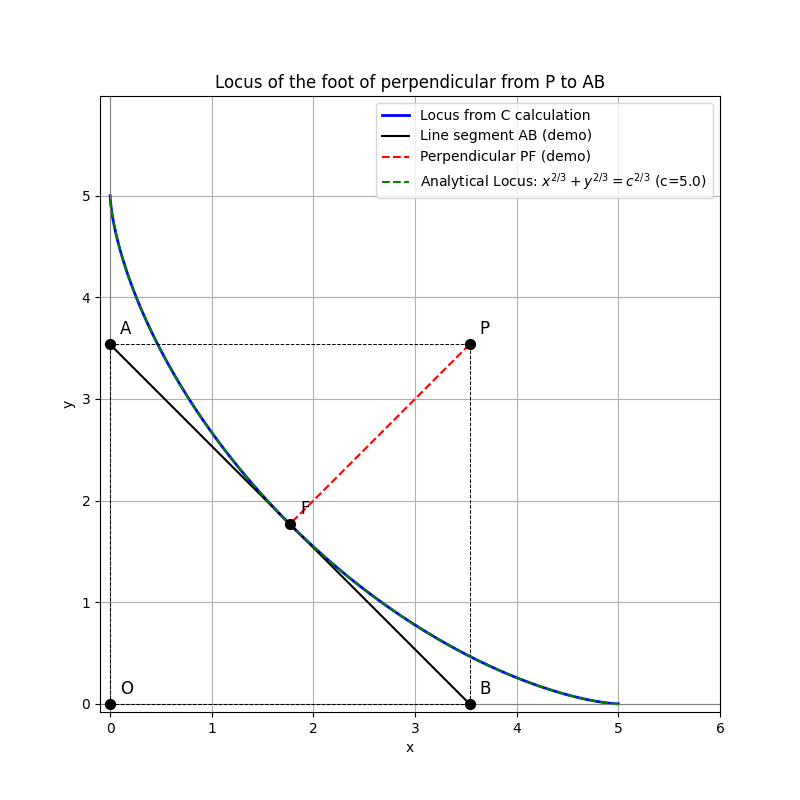
\includegraphics[width=0.7\columnwidth]{../figs/fig1.png}
\caption{}
\label{fig:1}
\end{figure}
\end{frame}

\begin{frame}{Plot by Python only}
\begin{figure}[H]
\centering
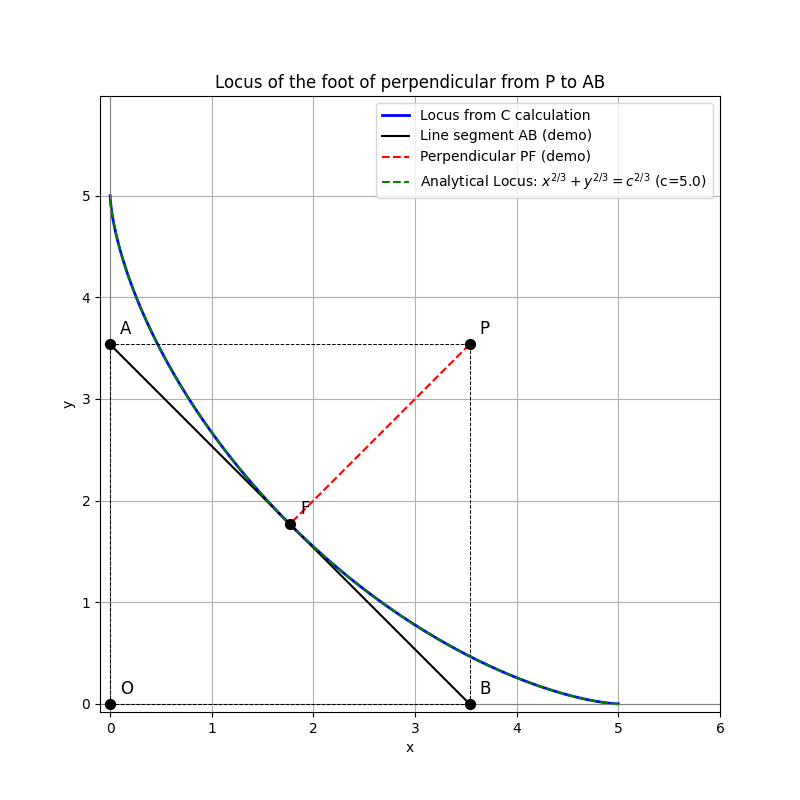
\includegraphics[width=0.7\columnwidth]{../figs/fig2.png}
\caption{}
\label{fig:2}
\end{figure}
\end{frame}

\end{document}
